%%%%%%%%%%%%%%%%%%%%%%%%%%%%%%%%%%%%%%%%%%%%%%%%%%%%%%%%%%%%%%%%%%%%%%%%%%%%%%%%
%2345678901234567890123456789012345678901234567890123456789012345678901234567890
%        1         2         3         4         5         6         7         8

% \documentclass[a4, 10 pt, conference]{ieeeconf}  % Comment this line out if you need a4paper

\documentclass[a4paper, 10pt, conference]{ieeeconf}      % Use this line for a4 paper

\IEEEoverridecommandlockouts                              % This command is only needed if 
                                                          % you want to use the \thanks command

\overrideIEEEmargins                                      % Needed to meet printer requirements.

% See the \addtolength command later in the file to balance the column lengths
% on the last page of the document

% The following packages can be found on http:\\www.ctan.org
%\usepackage{graphics} % for pdf, bitmapped graphics files
%\usepackage{epsfig} % for postscript graphics files
%\usepackage{mathptmx} % assumes new font selection scheme installed
%\usepackage{times} % assumes new font selection scheme installed
%\usepackage{amsmath} % assumes amsmath package installed
%\usepackage{amssymb}  % assumes amsmath package installed
\usepackage{multicol}
\usepackage{tcolorbox}
\usepackage{cuted,tcolorbox,lipsum}
\usepackage{xcolor}

\title{\LARGE \bf
Introduction to Machine Learning (SS 2024)\\ Project: Programming Project
\vspace{-3em}
}


%\author{Someone Anyone$^{1}$ and Xiang Zhang$^{2}$% <-this % stops a space
%}


\begin{document}


\maketitle
\vspace{-3em}
\thispagestyle{empty}
\pagestyle{empty}

\begin{strip}
\begin{tcolorbox}[
size=tight,
colback=white,
boxrule=0.2mm,
left=3mm,right=3mm, top=3mm, bottom=1mm
]
{\begin{multicols}{2}% replace 3 with 2 for 2 authors.

\textbf{Author 1}\\
Last name: Rieser\\
First name: David\\
Matrikel Nr.: 12141689\\

\columnbreak

\textbf{Author 2}\\
Last name: Sillaber\\
First name: Cedric\\ 
Matrikel Nr.: 12211124\\ 

\columnbreak

\end{multicols}}
\end{tcolorbox}
\end{strip}

%%%%%%%%%%%%%%%%%%%%%%%%%%%%%%%%%%%%%%%%%%%%%%%%%%%%%%%%%%%%%%%%%%%%%%%%%%%%%%%%

\section{Introduction}
\label{sec:intro}
The task of this project is to implement machine learning models to detect fraudulent transactions. 
The problem type is a binary classification task. Based on the timestamp, amount, and 28 additional features, the model should predict if a transaction is fraudulent or not. 
The dataset consists of 227,845 instances with 30 features and a flag indicating if the transaction is fraudulent. The dataset is highly imbalanced, with 0.173\% of the transactions being fraudulent. There is no information about the 28 features, so it is not clear what they represent. 

As the dataset is labeled, we can use supervised learning to solve this problem. We decided to use three methods for this problem. 
The first choice was to use a neural network. Neural networks can extract the most important features from the data and learn complex patterns. 
The second choice was a decision tree. To achieve even better results, we also tried a random forest classifier.

\section{Implementation / ML Process}
\label{sec:methods}
As mentioned in the introduction, the dataset is highly imbalanced. There are 227,845 data points, and less than 500 are fraudulent, which is about 0.173\% of the dataset. So, when splitting the dataset into train and validation sets, we have to work with only a few fraud cases. 
A naive implementation of the neural network was not able to detect frauds correctly. With an accuracy of 99.83\%, most likely, the frauds were not detected. 
To solve this problem, we decided to do simple data augmentation. As other methods were not adequate, we simply duplicated the fraudulent transactions. 
This was done as follows: The dataset was split into train and validation sets. Then the fraudulent transactions in the train set were duplicated randomly by a factor. 
Using this augmentation method, it was possible to give the frauds more weight in the train set, without changing the validation set. 
Additionally, we scaled the data using a normalization method. This functionality is achieved by calling scikit-learn's `StandardScaler`. 

% The timestamp in the dataset was removed as it is most likely not important. 
For the problem, we used two methods: Multilayer Perceptron and Decision Tree. 

\subsection{Multilayer Perceptron}

The neural network is based on `pytorch`'s `nn.Module`. For the network, there are three layers: 
an input layer with 30 nodes, a hidden layer with a dimensionality of 94, and a learning rate of 0.0004301150216793739. 
The activation function is a ReLU function. The output layer has one node and a sigmoid activation function.

A neural network is suitable for this problem as it can learn complex patterns and extract the most important features from the data. 
We don't have any information about the features, so a neural network is a good choice. The programmer does not have to make any choices concerning the features. 
The dataset contains labeled data, so supervised learning and thus neural networks seem a good option.

The choice of hyperparameters was really important and made a difference. In this case, the hyperparameters were the factor used for the data augmentation, the number of nodes in the hidden layer, learning rate, and learning epochs. 
To find the best hyperparameters, we used a brute force method to train using randomly selected parameters. The parameters were randomly selected from a specified range. 
Given the results, the best hyperparameters were chosen. 
The final hyperparameters are: factor for data augmentation: 100, number of nodes in hidden layer: 94, learning rate: 0.0004301150216793739, learning epochs: 45.

\subsection{Decision Tree}

The Decision Tree is based on the `sklearn` library. 

Decision Trees are suitable for this problem as it can easily divide the multi-dimensional space given by the amount of features into distinct sections each with a given probability of being a fraud. For this the decision 


This left us with the following hyperparameters: The maximum depth of the tree, the criterion on when to split the nodes, how to split the nodes, and the maximum amount of features. 



\subsection{Random Forest}

We further tested a modification of decision trees - the random forest classification. This method is based on the decision tree but uses multiple trees to improve accuracy. 
The accuracy was about 99.959\%, and the model was able to detect the frauds. This is about the same as the accuracy of the decision tree.

\section{Results}
\label{sec:results}
During the training of the MLP model, the dataset was split into a training set and a validation set. The training set consisted of 70\% of the data, while the remaining 30\% was allocated to the validation set.

The final accuracy achieved on the training set was 99.9999\%, demonstrating excellent performance in learning from the data. On the validation set, the model achieved an accuracy of 99.9415\%, indicating robust generalization to unseen data.

Moreover, the ROC AUC score obtained on the validation set was 96.62923\%. This metric signifies the model's ability to distinguish between fraudulent and legitimate transactions, with an accuracy of detecting approximately 96.62923\% of fraudulent activities.

The figure below shows the training loss for the MLP. In the first few iterations, the loss is decreasing rapidly, but this trend slows down. This is the typical loss curve for an MLP. 
\begin{center}
  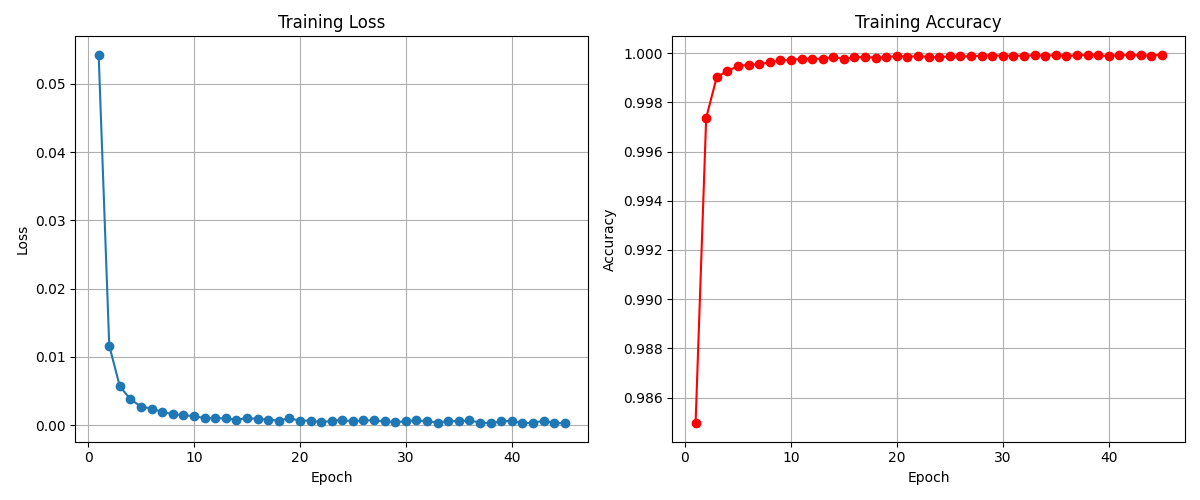
\includegraphics[width=8.5cm]{../data/mlp-plot.png} \label{mlp-plot}
\end{center}

Using the test set on the JupyterHub, which consisted of different data, showed only ROC. The ROC for the train set was 99.2065\%, and the test score was 98.7157\%. This is a solid result.

The decision tree has a validation accuracy of 99.96\%. The train accuracy is about... % to insert

As a naive baseline predictor, we present a model that only outputs 0, meaning no fraud. 
Because the dataset is imbalanced and data augmentation does not affect the validation set, there are only a maximum of 0.15\% frauds in the validation set. 
Thus, the naive predictor has an accuracy of at least 99.85\%. 
Both implementations are significantly better than the naive baseline predictor. The decision tree and random forest classification can detect frauds.

{\color{blue}
\begin{itemize}
	\item Describe the performance of your model (in terms of the metrics for your dataset) on the training and validation sets with the help of plots or/and tables.
	\item You must provide at least two separate visualizations
          (plot or tables) of different things, i.e. don’t use a table
          and a bar plot of the same metrics. At least three
           visualizations are required for the 3 person team.
\end{itemize}
}

\section{Discussion}
\label{sec:discuss}
As mentioned above, our models are significantly better than a model that only predicts no fraudulent transactions.

The decision tree can pretty accurately classify both fraud and non-fraud. 
In testing it mispredicted 13 non-frauds of 45493 total and 1 frauds of 73 total.
This results in a testing accuracy of 0.9996927735960851 which is way above the baseline predictor.

A reason we think the model perfomed so well is that frauds usually have something that makes them stick out. 
This enables the decision tree to learn which tresholds for features indicate a fraud. 
This theory is also supported by the structure of the decision tree as it only uses about a third of the features defined in the dataset.
The model is also remarkably small, coming in at a little more than 2KB in pure text form.

We also tried removing the timestamp from the dataset since the time of a transaction likely does not hold any information about its fraudulence, but it did not improve the model's accuracy and caused problems with the test harness on JupyterHub.

The neural network approach did not work as well as the decision tree on the train and validation set. However, the ROC for the dataset on the JupyterHub was really good and even better than the decision tree.
 This could have been improved by further hyperparameter optimization as well as experimenting with more hidden layers. The model size is also notably small with only 14 KB as a pickle jar. 


{\color{blue}
\begin{itemize}
	\item Analyze the results presented in the report (comment on what contributed to the good or bad results). If your method does not work well, try to analyze why this is the case.
	\item Describe very briefly what you tried but did not keep for your final implementation (e.g. things you tried but that did not work, discarded ideas, etc.).
	\item How could you try to improve your results? What else would you want to try?
\end{itemize}
}

\section{Conclusion}
\label{sec:con}
Overall, while the decision tree excels in both accuracy and model size efficiency, the neural network demonstrates a strong potential with superior ROC scores.
Both models significantly outperform a naive baseline predictor. However, due to the limited number of fraudulent transactions in the dataset, the models are not yet perfect. 
Before deploying these models in a real-world application, further experimentation and optimization are necessary.

Our main takeaway was the contrast between traditional coding and machine learning. 
Machine learning involves lots of trial and error to identify the right model and optimal hyperparameters. 
While theoretical knowledge is essential for building a foundational understanding of the model and knowing which techniques to apply, 
experimenting with different configurations is crucial.

{\color{blue}

%{\color{blue}
%\begin{itemize}
%  \item Finally, describe the test-set performance you achieved. Do not optimize your method based on the test set performance!
%  \item Write a 5-10 line paragraph describing the main takeaway of your project.
%  \end{itemize}
%  \end{itemize}
%
%\end{itemize}

%}

%%%%%%%%%%%%%%%%%%%%%%%%%%%%%%%%%%%%%%%%%%%%%%%%%%%%%%%%%%%%%%%%%%%%%%%%%%%%%%%%

\end{document}
